\documentclass[11pt,a4paper]{jsarticle}
%
\usepackage{amsmath,amssymb}
\usepackage{bm}
\usepackage{ascmac}
\usepackage[dvipdfmx]{graphicx}
%
\setlength{\textwidth}{\fullwidth}
\setlength{\textheight}{40\baselineskip}
\addtolength{\textheight}{\topskip}
\setlength{\voffset}{-0.2in}
\setlength{\topmargin}{0pt}
\setlength{\headheight}{0pt}
\setlength{\headsep}{0pt}
%
\newcommand{\writtenBy}[1]{\begin{flushright}文責: #1\end{flushright}~}
\newcommand{\divergence}{\mathrm{div}\,}  %ダイバージェンス
\newcommand{\grad}{\mathrm{grad}\,}  %グラディエント
\newcommand{\rot}{\mathrm{rot}\,}  %ローテーション
%
\title{競技プログラミング班 活動報告書}
\author{服部瑠斗 小村漱一朗 中野海人 稲垣和真 浜田直弥 西見元希 石川琉聖}
\date{\today}
\begin{document}
\maketitle
%
%
\section{活動の概要}
\writtenBy{稲垣 和真}
本プロジェクトは、競技プログラミングを通してプログラミングにおけるアルゴリ
ズムの知見を深めるために発足した。競技プログラミングに用いたツールはAtCoderであ
る。AtCoderのBeginner Contestや班内の活動内で開催したバーチャルコンテストを通し
て実際に問題を解き、その解法を活動で共有し、お互いの知見を高めたり、いろいろな
アルゴリズムの手法について会員が解説し、理解を深めるというものである。以上の2点
を主として本プロジェクトは活動した。

\section{競技プログラミングについて}
\writtenBy{稲垣和真}
競技プログラミングとは、解くべき問題が与えられ、その問題を解くプログラムを、早
く正確に解き、正解数や解くまでにかかった時間などを競う競技である。具体的には以
下の5つの要素からなる。
\begin{itemize}
    \item {\bf 問題文}
        \par
        解くべき問題の内容が記されている。
        \par
    \item {\bf 制約}
        \par
        問題文で出てきた数値や文字列に、どのような制約が与えられているかが記さ
        れている。
    \par
    \item {\bf 入力}
        \par
         入力は、標準入力にどのような形式で文字列を与えるかが記されている。
    \par
    \item {\bf 出力}
        \par
        標準出力にどのような形式で与えるかの条件が記されている。
    \par
    \item {\bf 入出力例}
        \par
        実際にプログラムに与えられる入力と、プログラムが出力すべき文字列が記されている。
\end{itemize}
\section{学習内容}

\subsection{アルゴリズム}
この班では以下の2つのアルゴリズムを学習した.
\begin{itemize}
    \item 深さ優先探索(dfs)
    \item 累積和
\end{itemize}

\subsubsection{深さ優先探索}
深さ優先探索とは、全探索を行うアルゴリズムの種類の一つです。
競技プログラミングでは主に、状態の遷移が分岐するような処理の実装に用いられています。
深さ優先探索の特徴として、与えられた状態の深さに注目して探索を行うという点が挙げられます。
また深さ優先探索を用いるメリットとして、再帰を用いて実装した場合コードがシンプルに記述することが出来るという点が挙げられます。

深さ優先探索の実装例

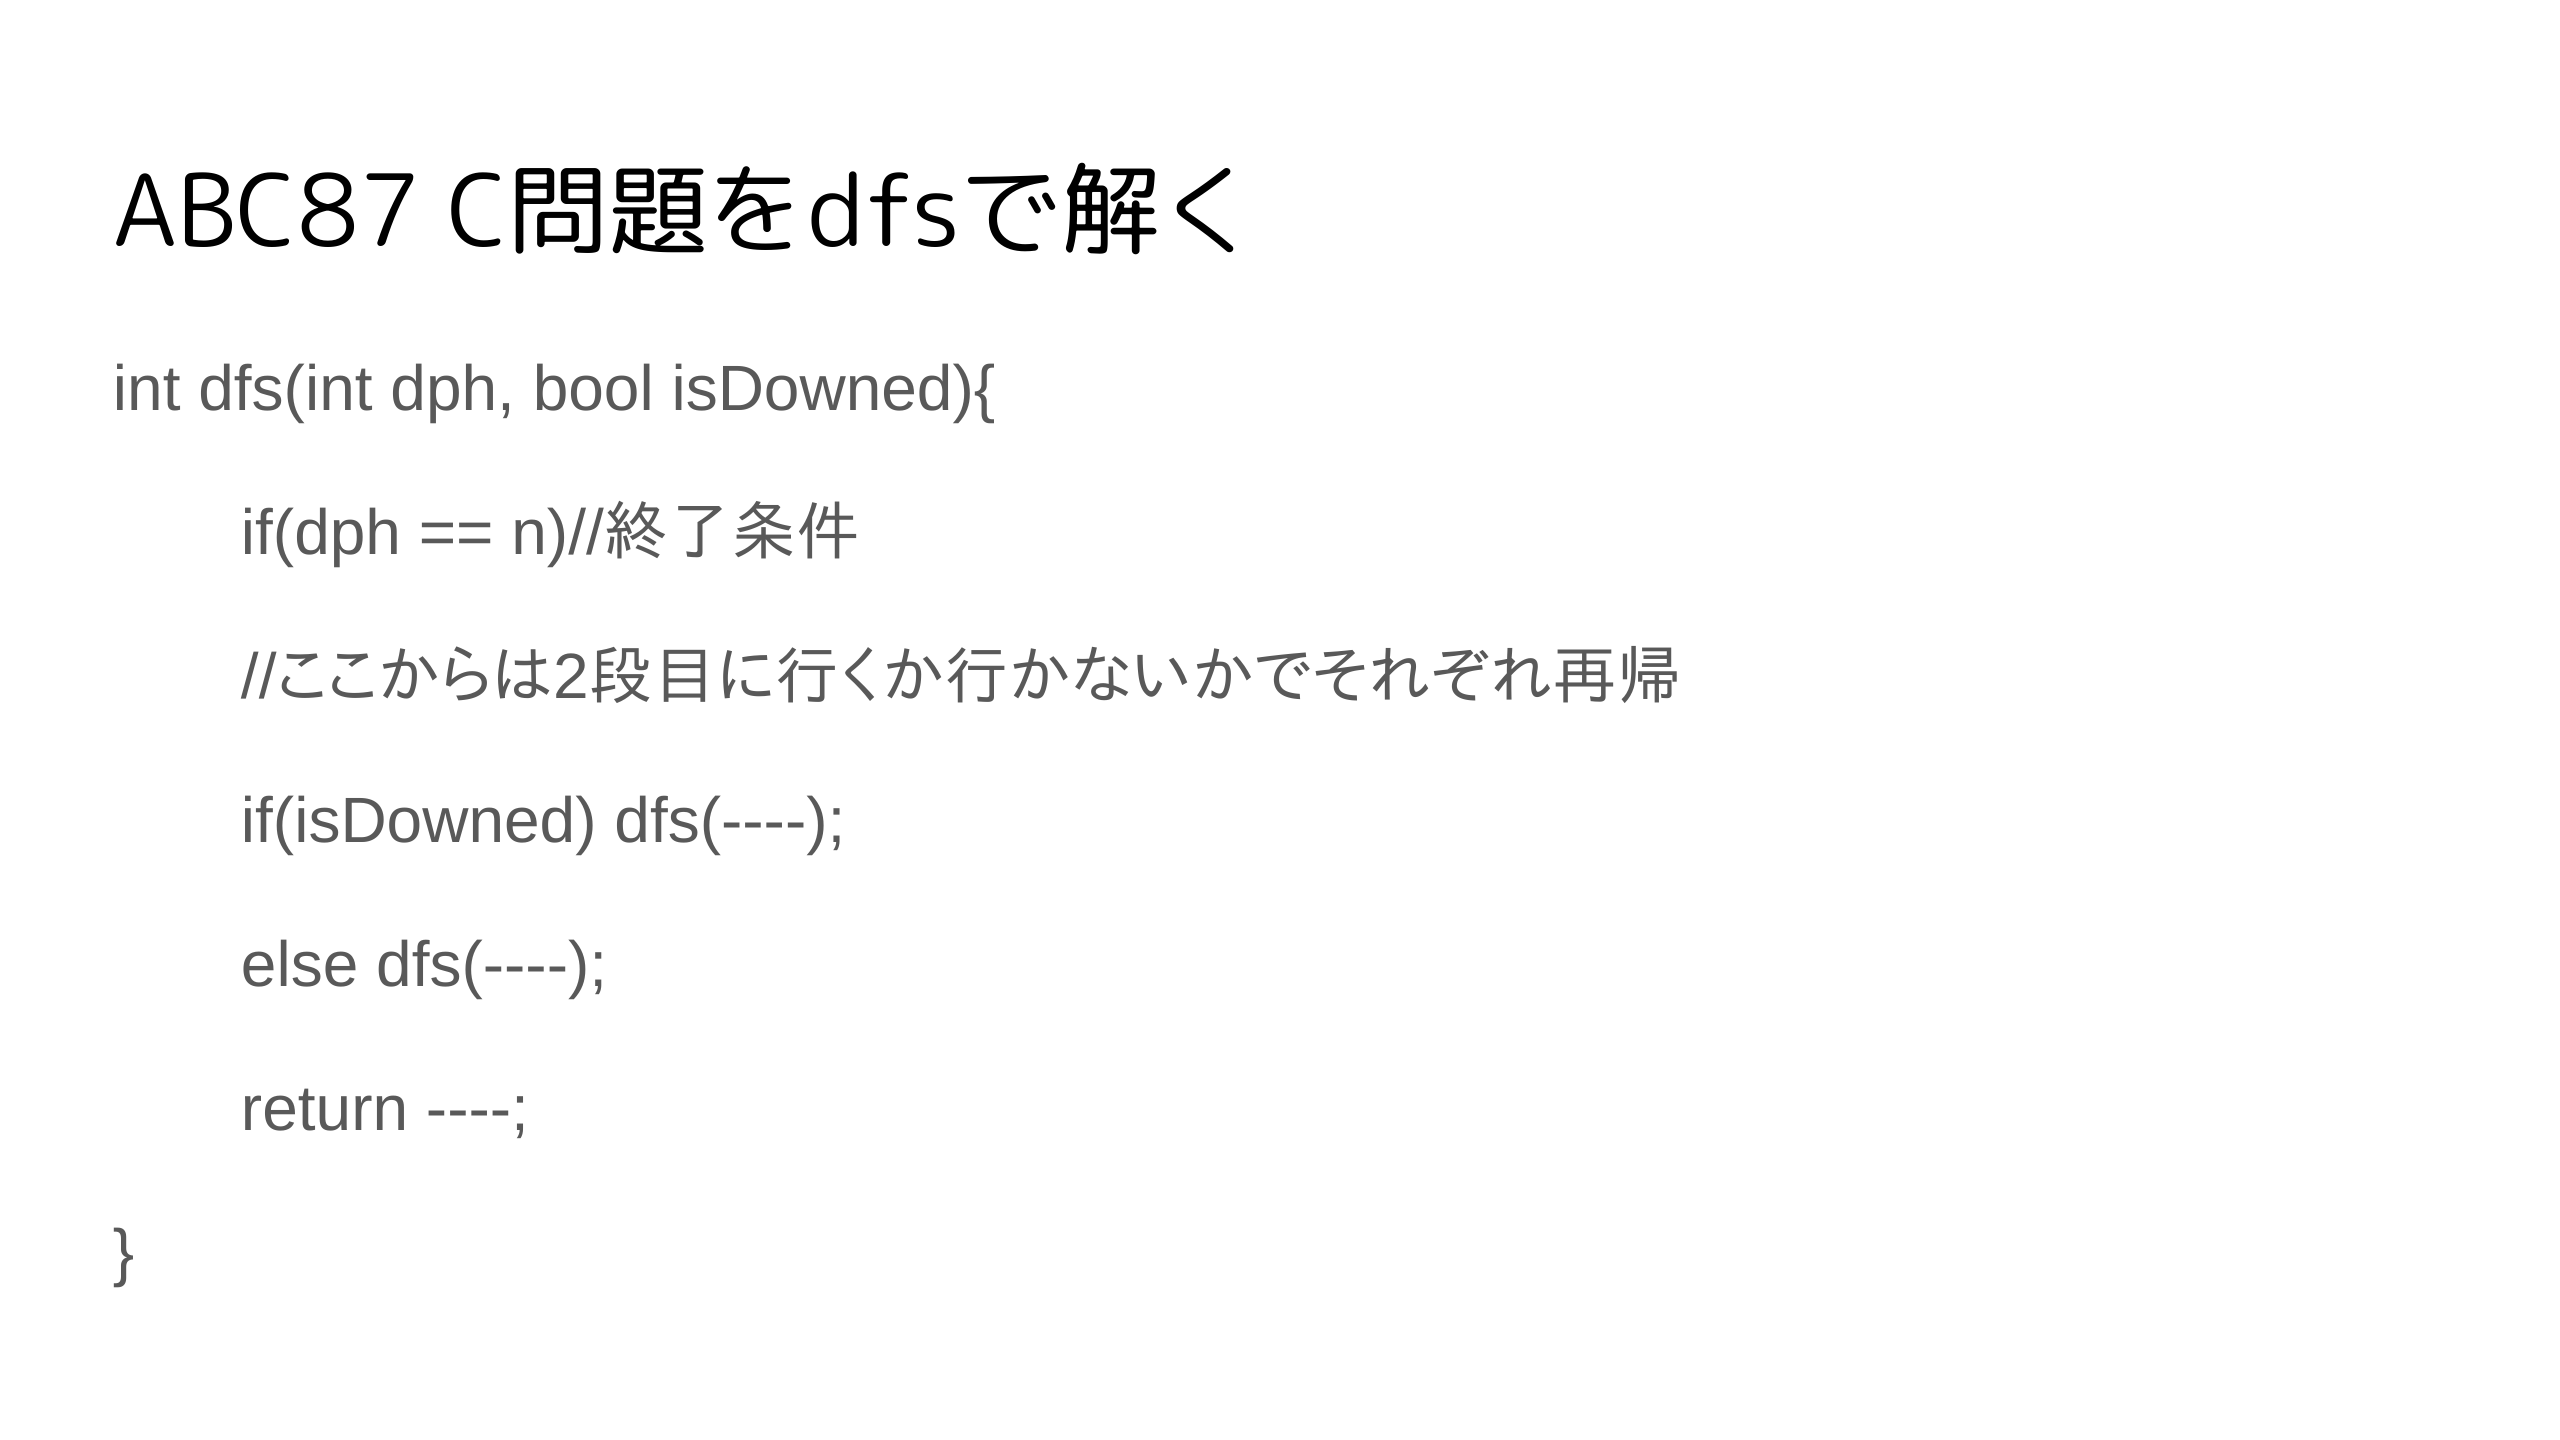
\includegraphics[width=10cm]{dfs.png}

\subsubsection{累積和}
累積和とは、計算量(オーダー)を圧縮するために用いられるアルゴリズムの種類の一つです。
競技プログラミングでは主に、配列上の区間の総和を求める処理の実装に用いられています。
累積和の特徴として、前処理を行うことによって元々の配列が保持している情報に加えてある区間の総和も求めることが出来るという点が挙げられます。

累積和の実装例.

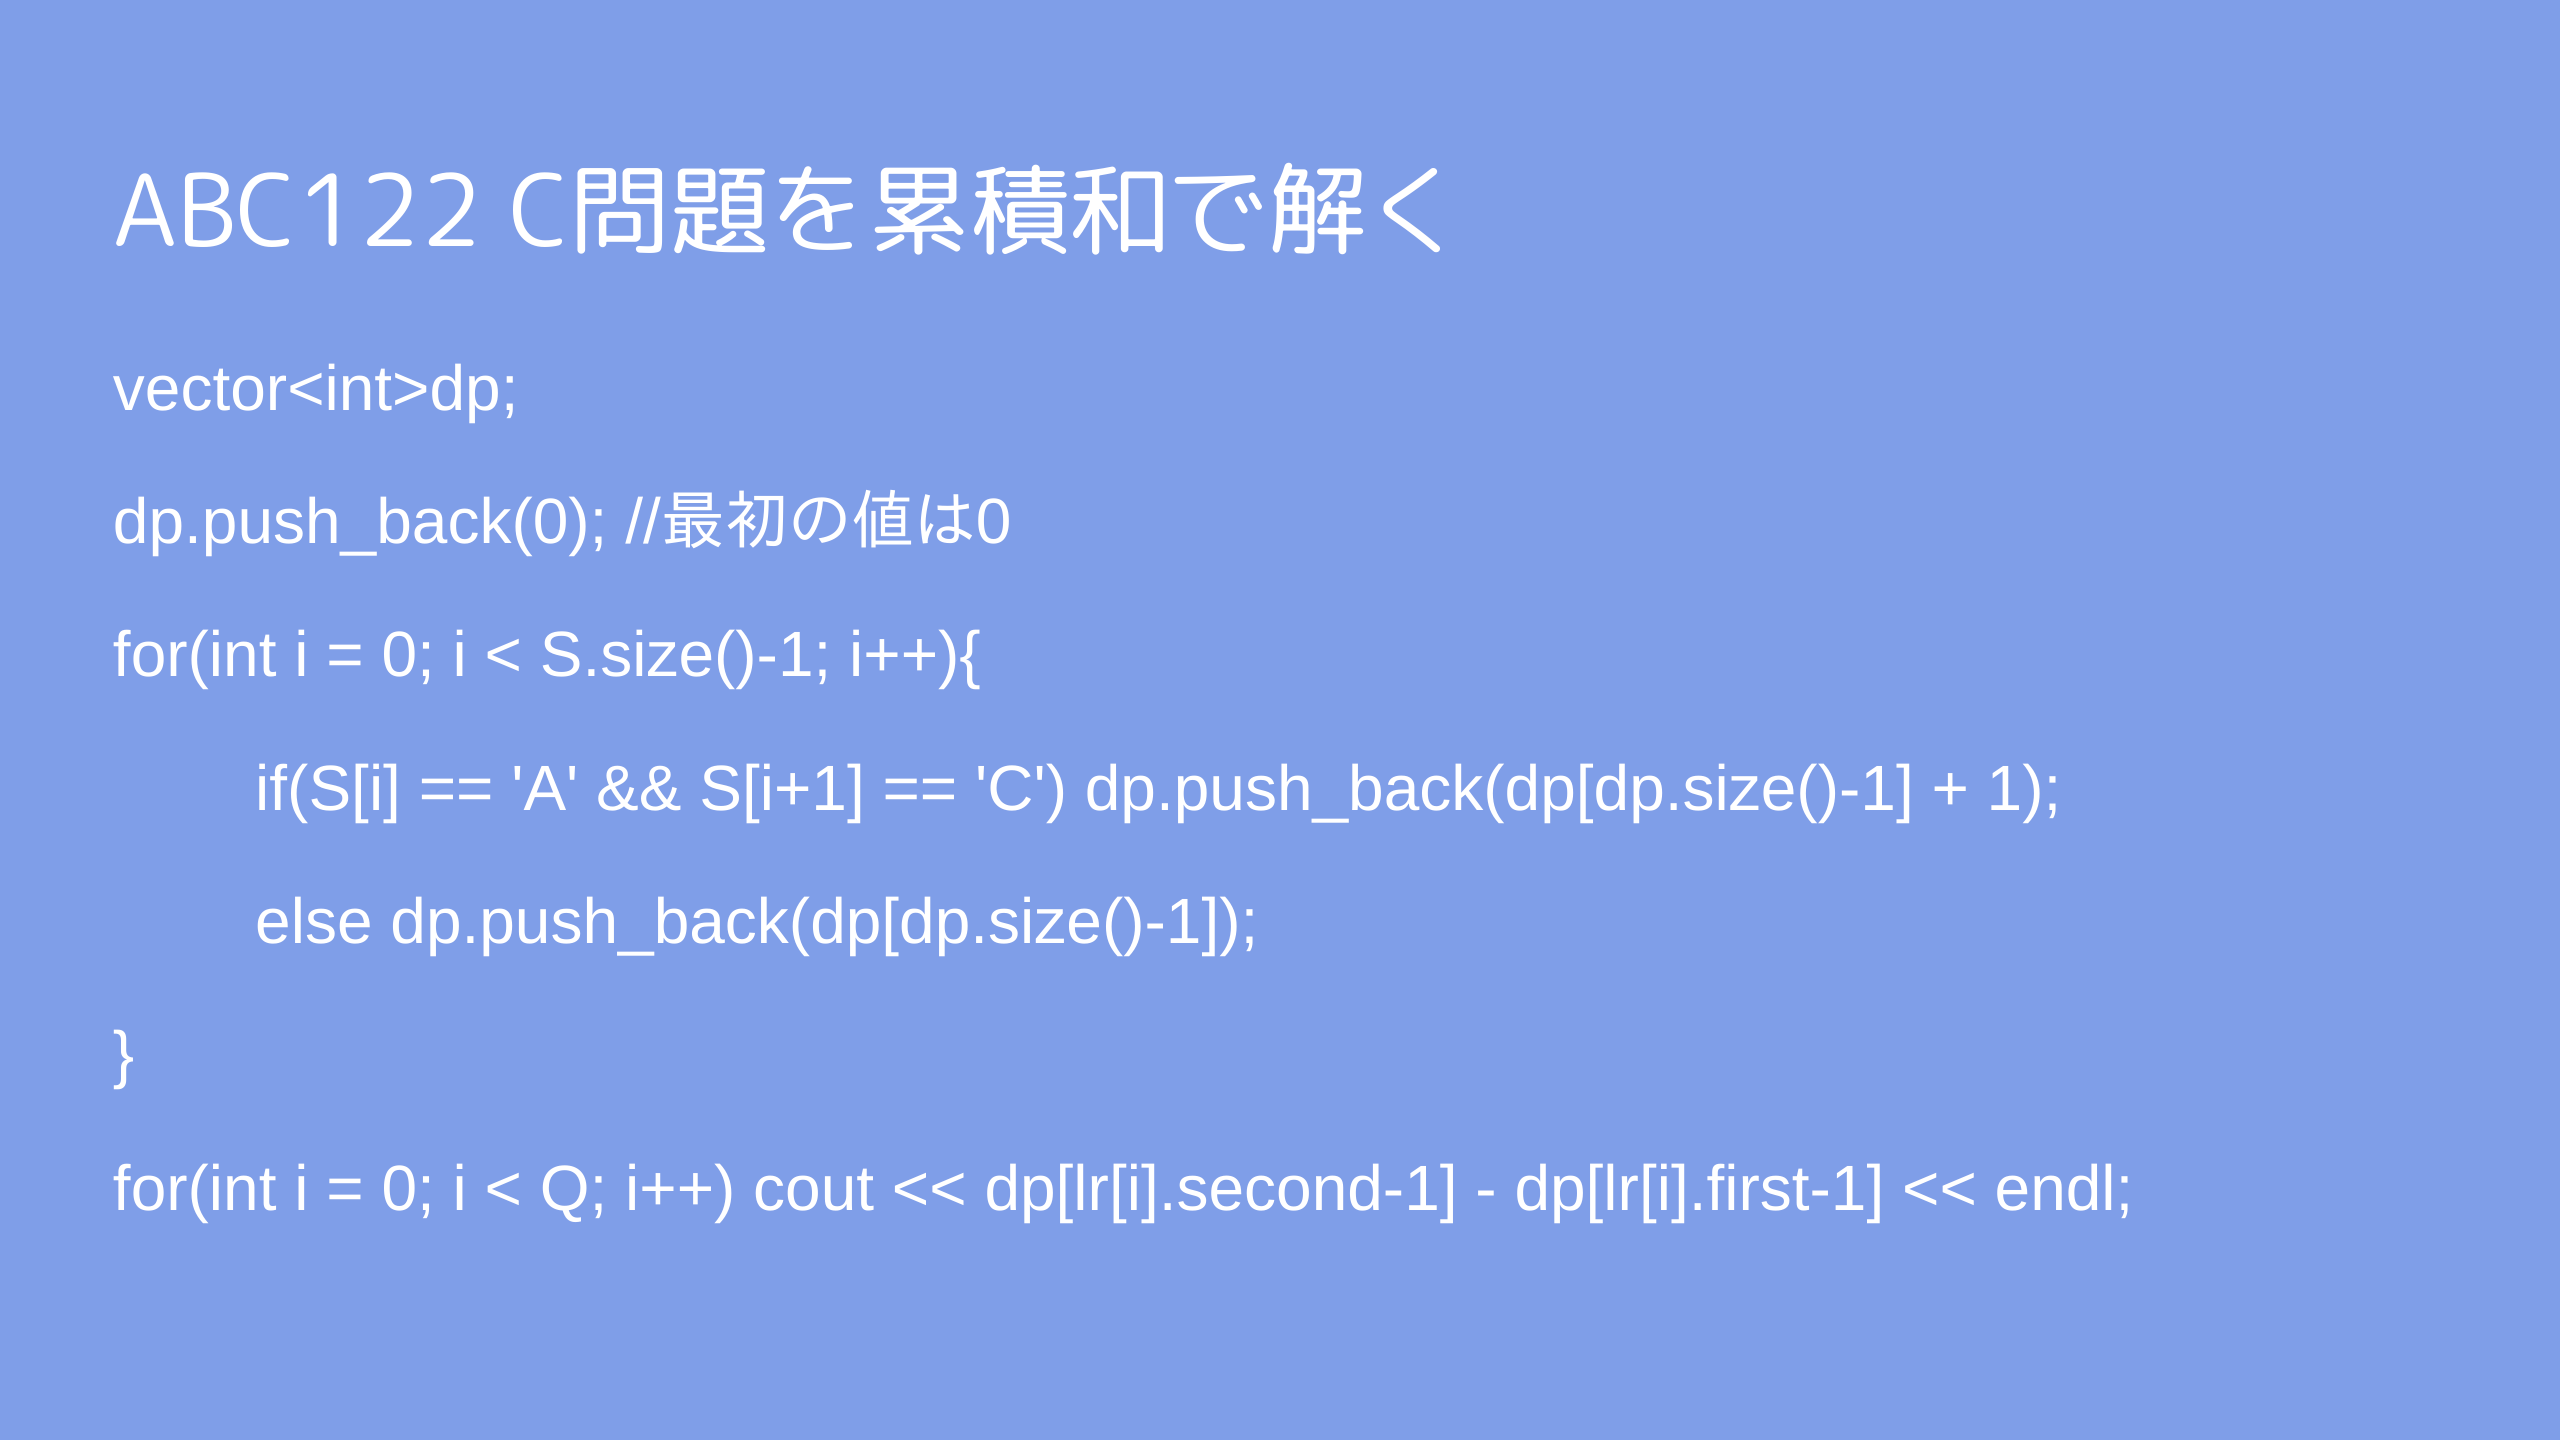
\includegraphics[width=10cm]{ruisekiwa.png}

\subsection{競技プログラミングにおけるテクニック}
\section{活動で得られたもの}
\section{問題点}
\section{展望}
\begin{thebibliography}
    \texttt{https://book.mynavi.jp/manatee/detail/id=56242}
\end{thebibliography}




%
%
\end{document}
